\FILE{section/nlp.tex}

\subsection{NLP}


Natural Language Processing is one of the first services offered by
many cloud providers. This is motivated by analyzing large amounts of
text in volume and number and deriving automated content from
it. Popular services include keyword extraction, sentiment analysis,
auto summary, and translation.  The services are offered often by large
cloud providers such as Google, IBM Watson, and Amazon to consumers for
a fee. In addition, such tools are also offered as stand-alone
components and software packages.

As many such services are offered by the different providers, and
standalone components and software packages exist, it allows us to use
them to test the framework for implementing hybrid and multi-cloud
analytics services. We can therefore analyze each of their APIs and
compare functionality as well as the performance characteristics of
local as well as cloudservices. We also can test our design of the
cloud service catalog to identify the strategy of dynamically
locating similar services and integrating them into a service offering.

For our work, we have restricted our analysis to two cloud services
from Amazon and Google, while the integration of a third from Amazon
is under development. Furthermore, we have only considered the
translation service as it provides an easy abstraction of a service
that translates a text from a source language to a target language:

\smallskip
\begin{Verbatim}[fontsize=\small]
def translate(text, source_langauge, target_langauage, ...):
    ...
    return translation
\end{Verbatim}
\smallskip

Each of the services is implemented with a different API. We contrast
the API in Figure ... showcasing the difference in invoking a
translation service as well as showcasing the result of the JSON
response of such a service.


If the interface is on purpose defined differently a switch will cost
extra work and may therefore not be in the interest of the users.  It
is obvious that users can benefit from a uniform implementation of
this API in order to easily switch from one provider to the other.
Naturally, the cloud providers typically do not have any interest in
providing such a uniform API as it may entice the customers to switch
service providers.

Hence a multicloud CLI implementation may look as follows, where the
provider flag is used to distinguish the different cloud providers
offering the translation service. Naturally, we could also utilize a
local translation program such as offered from industry and easily make
this example a hybrid service that also integrates with a local
implementation.

%\resizebox{1.0\columnwidth}{!}{
\begin{Verbatim}[fontsize=\small]
cms nlp translate --provider=google --from=en --to=de hello world
cms nlp translate --provider=aws --from=en --to=de hello world
cms nlp translate --provider=local --from=en --to=de hello world
\end{Verbatim}
%}


As each of the services returns natively a different output, it is
beneficial to unify the output and create a mapping from the
originating service to the output. An example of such a uniform output is given next.


\begin{Verbatim}[fontsize=\small]
{'date': '05/02/2022 14:45:45',
 'input': 'hello world',
 'input_language': 'en',
 'output': 'Hallo Welt',
 'output_language': 'de',
 'provider': 'aws',
 'time': 0.2641}
\end{Verbatim}


Other parameters such as service region can easily be integrated in
this example. Furthermore, it is obvious that the commandline
application underlying API can be used in a REST service
implementation and can be generalized into different REST service
frameworks. For our implementation, we have used FastAPI and used the
closest regional service center to our location.

The result of the translation that simply translates a text from
German ``Hallo Welt'' to English ``Hello World'' is showcased for 100
invocations in Figure~\ref{fig:nlp-performance}. 


\begin{figure}[htb]

\centering
%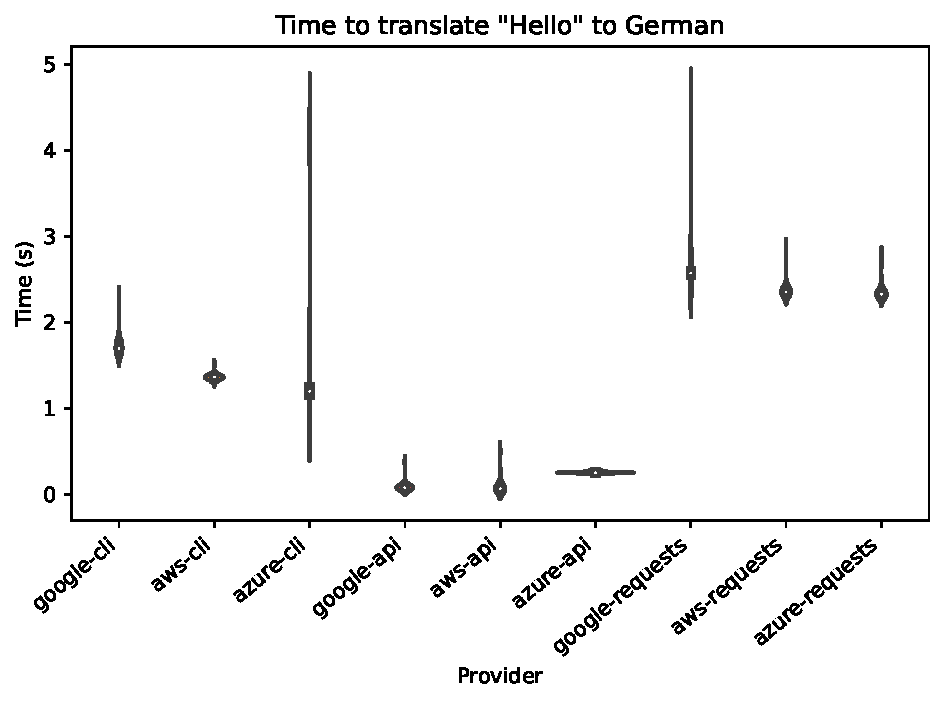
\includegraphics{images/nlp-benchmark.pdf}
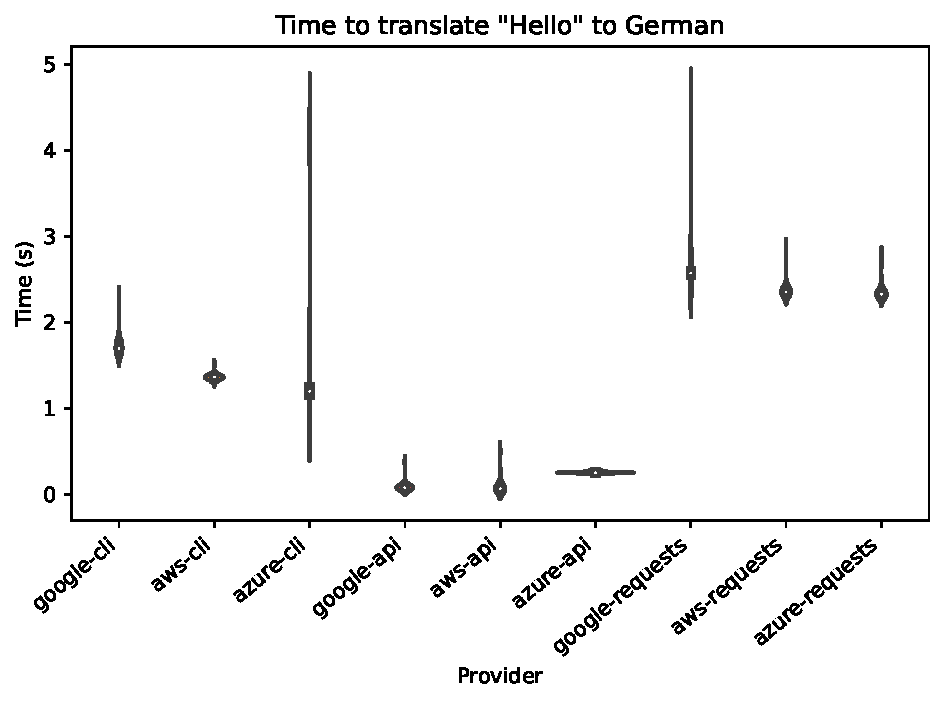
\includegraphics[width=1.0\columnwidth]{images/nlp-benchmark.pdf}

\caption{Natural Language processing performance for a single
         word translation.}
\label{fig:nlp-performance}

\end{figure}


Such a performance analysis could be performed based on customer needs
and could indicate factors for preferential service choices. This may
include besides time other factors such as cost and quality, or even
service level reliability at different times.

For us, we found that for the short query we used the service
offered by AWS to translate the text was on average 
faster when executed from Bloomington, IN to the closest service
centers for the provider.


\begin{table*}[htb]

\caption{Comparision of the time it takes on average to translate the word hello from English to German}

\begin{tabular}{lrrrrrrrrr}
 & google-cli & aws-cli & azure-cli & google-api & aws-api & azure-api & google-requests & aws-requests & azure-requests \\
 \hline
count & 20.000000 & 20.000000 & 20.000000 & 20.000000 & 20.000000 & 20.000000 & 20.000000 & 20.000000 & 20.000000 \\
mean & 1.737850 & 1.369900 & 1.365600 & 0.094800 & 0.099300 & 0.257150 & 2.681500 & 2.381500 & 2.352550 \\
std & 0.134381 & 0.043240 & 0.664569 & 0.066135 & 0.104365 & 0.009292 & 0.429593 & 0.111200 & 0.100339 \\
min & 1.643000 & 1.297000 & 1.120000 & 0.069000 & 0.064000 & 0.245000 & 2.532000 & 2.330000 & 2.299000 \\
25\% & 1.675250 & 1.346750 & 1.162750 & 0.075000 & 0.066750 & 0.251000 & 2.556750 & 2.349250 & 2.316500 \\
50\% & 1.695000 & 1.366500 & 1.198500 & 0.079000 & 0.067500 & 0.255000 & 2.574000 & 2.354000 & 2.329500 \\
75\% & 1.749000 & 1.378750 & 1.246750 & 0.085750 & 0.069250 & 0.259500 & 2.592750 & 2.367750 & 2.341500 \\
max & 2.266000 & 1.520000 & 4.170000 & 0.374000 & 0.497000 & 0.280000 & 4.481000 & 2.848000 & 2.766000 \\
\hline
\end{tabular}
\end{table*}

